\documentclass[12pt,a4paper,titlepage]{report}

\usepackage[titletoc]{appendix}
\usepackage[nottoc]{tocbibind}
\usepackage{fancyhdr}
\usepackage{graphicx}
\usepackage[left=3.5cm, right=2.5cm, top=3.0cm, bottom=2.5cm]{geometry}
\usepackage{newsec}
\usepackage{titlesec}
\usepackage{float}
\usepackage{amsmath}
\usepackage{array}
\usepackage{booktabs}
\usepackage{longtable}
\usepackage{multirow}
\usepackage{url}
\usepackage{tikz}
\usepackage{xcolor}
\usepackage{listings}
\usepackage[hidelinks]{hyperref}
\usetikzlibrary{arrows.meta,positioning,fit,shapes.geometric,shapes.symbols}

\titleformat{\chapter}[display]
{\normalfont\Large\bfseries\centering}{\chaptertitlename\ \thechapter}{20pt}{\Large}
\titlespacing*{\chapter}{0pt}{-10pt}{16pt}

\newcommand{\ReportTitle}{FLUIDWORKS: REAL-TIME CFD VISUALIZATION PLATFORM}
\newcommand{\ReportTitleMixed}{FluidWorks: Real-Time CFD Visualization Platform}
\newcommand{\LegacyProductName}{AeroFlow}

\definecolor{codebg}{RGB}{247,248,250}
\definecolor{codeframe}{RGB}{210,214,220}
\definecolor{codeblue}{RGB}{22,90,180}
\definecolor{codegreen}{RGB}{20,120,80}
\definecolor{codegray}{RGB}{110,110,110}

\lstdefinestyle{fluidworksstyle}{
backgroundcolor=\color{codebg},
basicstyle=\ttfamily\footnotesize,
breaklines=true,
captionpos=b,
commentstyle=\color{codegreen},
frame=single,
framerule=0.3pt,
rulecolor=\color{codeframe},
keywordstyle=\color{codeblue}\bfseries,
numbers=left,
numbersep=8pt,
numberstyle=\tiny\color{codegray},
showstringspaces=false,
tabsize=4
}

\lstset{style=fluidworksstyle}

\begin{document}

\titlepage
\thispagestyle{empty}
\begin{center}
\Large \textbf{FLUIDWORKS: REAL-TIME CFD\\VISUALIZATION PLATFORM}\\[1.6cm]
\large \textit{The Mini Project report submitted in partial fulfillment of the
requirements for the award of the degree of}\\[1cm]
{\huge {$\mathfrak {Bachelor\; of\; Technology}$}}\\[.5cm]
\textit{in}\\[.5cm]
{\Large \bf \itshape{{Artificial Intelligence \& Machine Learning}}}\\[1cm]
\large \textit{by}
\vskip1.0cm
\large{Abhinav Manoj} (\small{Reg. No. MCE23AIM003})\\
\large{Niranjan J} (\small{Reg. No. MCE23AIM047})\\
\large{Abhiram Vijaykumar Kaimal} (\small{Reg. No. MCE23AIM004})\\
\large{Rohan Tom Reji} (\small{Reg. No. MCE23AIM052})\\
\vskip1.0cm
\includegraphics[height=5cm]{college_logo-removebg.png}\\
\vspace{1cm}
\large \bfseries{Marian Engineering College}\\
\large \bfseries{Trivandrum}\\
\large \bfseries{Kerala}\\
\vspace{1.5cm}
\large \bfseries{March 2026}\\
\end{center}

\clearpage
\thispagestyle{empty}
\begin{center}
\Large \bfseries{DEPARTMENT OF ARTIFICIAL INTELLIGENCE \& MACHINE LEARNING}\\
\large\bfseries{Marian Engineering College}\\
\large \bfseries{Kazhakuttom, Trivandrum - 695582}\\
\vspace{1.0cm}
\includegraphics[height=6.0cm]{college_logo-removebg.png}\\
\vspace{1.5cm}
\textbf{CERTIFICATE}
\end{center}
\vspace{1.5cm}
This is to certify that the report entitled \textbf{``\ReportTitleMixed''} is a bonafide record
of the Mini Project presented by Abhinav Manoj (Reg. No. MCE23AIM003), Niranjan J (Reg. No. MCE23AIM047),
Abhiram Vijaykumar Kaimal (Reg. No. MCE23AIM004) and Rohan Tom Reji (Reg. No. MCE23AIM052) under our
supervision and guidance. The report has been submitted to the Department of Artificial Intelligence \& Machine Learning of Marian Engineering College, Kazhakuttom, Trivandrum in partial fulfillment of the award of the Degree of Bachelor of Technology in Artificial Intelligence \& Machine Learning, during the year 2025-2026.\\[.5cm]
\begin{center}
\line(1,0){435}
\end{center}
\vspace{1cm}
\begin{minipage}{.7\textwidth}
\begin{flushleft}
\textbf{Dr. Aswathy S U}\\
\itshape{Supervising Guide}\\
\itshape{Assistant Professor}\\
\itshape{Artificial Intelligence \& \\ Machine Learning}\\
\itshape{Marian Engineering College \\ Trivandrum}\\
\end{flushleft}
\end{minipage}
\begin{minipage}{1\textwidth}
\begin{flushright}
\vfill
\begin{flushleft}
\textbf{Prof. Balu John}\\
\itshape{Head of the Department}\\
\itshape{Artificial Intelligence \& \\ Machine Learning}\\
\itshape{Marian Engineering College \\ Trivandrum}\\
\end{flushleft}
\end{flushright}
\end{minipage}

\clearpage
\thispagestyle{empty}
\renewcommand\abstractname{ACKNOWLEDGEMENT}
\begin{abstract}
\vspace{1.5cm}
We express our sincere gratitude to our Principal \textbf{Dr. Abdul Nizar M.}, to \textbf{Prof. Balu John}, Head of the Department of Artificial Intelligence \& Machine Learning, and to our project coordinators and faculty members for their support throughout this work. We place special thanks on record to our supervising guide \textbf{Dr. Aswathy S. U} for the guidance, review, and encouragement that shaped this project. We also thank our friends and peers for their constant support during development, testing, and documentation.
\end{abstract}

\newpage
\renewcommand\abstractname{ABSTRACT}
\begin{abstract}
\vspace{1.5cm}
\ReportTitleMixed{} is a Unity-based desktop platform for real-time CFD-style visualization. The current project integrates a GPU wind-tunnel solver for external aerodynamics, an internal-flow pipeline with boundary-condition management and surface diagnostics, rotating-machinery and free-surface templates, runtime 3D model import, engineering-style visualization modes, and export-oriented UI workflows. The latest version emphasizes explicit solver control, readable visualization contracts, vehicle-aware aerodynamic estimates, and clearer internal-flow analysis. This updated report presents the present-day architecture of the repository, recent implementation changes, major modules, workflow diagrams, mathematical formulation, validation approach, limitations, and representative source code. Unlike the earlier shortened draft, this version is expanded as a full mini-project report with implementation commentary and code appendices so that it can serve both as a presentation document and as a technical record.
\end{abstract}

\newpage
\pagenumbering{roman}
\tableofcontents

\newpage
\listoffigures

\newpage
\listoftables

\newpage
\pagenumbering{arabic}
\setcounter{page}{1}

\pagestyle{fancy}
\setlength{\headheight}{15pt}
\fancyhead{}
\fancyfoot{}
\fancyhead[R]{\textit{\ReportTitleMixed}}
\fancyfoot[L]{\textit{Dept. of AI \& ML}}
\fancyfoot[R]{\textit{Marian Engineering College}}
\fancyfoot[C]{\thepage}
\renewcommand{\headrulewidth}{0.4pt}
\renewcommand{\footrulewidth}{0.4pt}

\chapter{Introduction}
\section{Overview}
FluidWorks is a real-time CFD-style visualization application built in Unity. The system is designed for interactive engineering study rather than certification-grade simulation. Instead of long offline solve cycles, the project focuses on quick iteration, readable flow visualization, runtime geometry loading, and directly accessible diagnostics. The current repository is no longer a small prototype. It contains a maintained external-aero wind-tunnel path, an internal-flow analysis path, dedicated visualization modules, scene templates, data export support, and a UI layer that manages simulation-specific controls.

The project still contains legacy namespaces and identifiers under the name \LegacyProductName{}, but the current product identity is \textbf{FluidWorks}. This updated report reflects the present repository rather than the earlier project state.

\section{Problem Statement}
Traditional CFD tools are powerful but are usually expensive in time, expertise, and workflow complexity. They require mesh generation, solver tuning, convergence monitoring, and domain-specific interpretation. For teaching, design review, and early-stage concept exploration, users often need something different: a system that can load a model quickly, run a visually meaningful flow approximation, and provide understandable metrics with minimal setup.

This project addresses the following problem:

\textit{How can a desktop application provide interactive, visually meaningful, and technically grounded fluid-flow analysis across multiple engineering scenarios while remaining fast enough for iterative use on commodity hardware?}

\section{Objectives}
The current implementation is aimed at the following objectives:
\begin{enumerate}
\item Build a unified desktop interface for multiple flow-analysis workflows.
\item Support runtime import of engineering geometry for immediate experimentation.
\item Provide a GPU-accelerated external-aero wind-tunnel pipeline.
\item Provide an internal-flow analysis path with opening detection and boundary assignment.
\item Convert solver fields into understandable views such as streamlines, slices, particles, and surface contours.
\item Expose engineering diagnostics and derived estimates in the UI.
\item Support report-friendly outputs through metrics export and visual capture.
\item Keep the software modular enough for future AI-assisted extensions.
\end{enumerate}

\chapter{Current Project Scope}
\section{Implemented Simulation Workflows}
The repository currently exposes multiple simulation templates through the UI and project-selection flow. Table \ref{tab:modes} summarizes the major implemented workflows.

\begin{table}[H]
\centering
\caption{Current simulation workflows in FluidWorks}
\label{tab:modes}
\begin{tabular}{p{3.0cm}p{4.2cm}p{6.3cm}}
\toprule
\textbf{Workflow} & \textbf{Primary Purpose} & \textbf{Current Notes} \\
\midrule
External Aero & Wind-tunnel style external flow around a vehicle or imported body & Most mature path; GPU Navier-Stokes grid solver, vehicle-aware outputs, multiple visualization contracts \\
Internal Flow & Pipe and duct style flow analysis & Mesh-driven boundary handling, opening classification, streamlines, surface pressure and friction visualization \\
Rotating Machinery & Rotor, fan, propeller, and turbine style visualization & Runtime geometry workflow with rotating-region controls and machine-oriented diagnostics \\
Free Surface & Dam-break or splash-style study & GPU particle-style free-surface path for educational and demonstrative use \\
\bottomrule
\end{tabular}
\end{table}

\section{Project Direction}
Although FluidWorks supports multiple templates, the repository notes and current codebase clearly establish the wind-tunnel path as the primary engineering workflow. The external-aero stack receives the strongest solver, diagnostics, and visualization attention. The latest internal-flow work extends this base with more explicit pipe boundary handling and body-surface diagnostics, which makes the project more complete as a teaching and demonstration platform.

\section{Need for the Present Report Revision}
The earlier version of this report was adequate as an overview, but it was too short for a complete mini-project submission and too light on implementation evidence. For academic review, the document should show not only the final features but also the engineering decisions, solver workflow, UI integration, and representative source code that make the project technically credible. This revision therefore adds more theory, implementation detail, validation commentary, and appendix listings from the current codebase.

\chapter{Literature and Technical Background}
\section{Interactive CFD as an Engineering Need}
Computational Fluid Dynamics is usually associated with high-fidelity finite-volume or finite-element solvers that require meshing, solver configuration, convergence tuning, and long execution times. Those tools are valuable for industrial design and certification, but they impose a significant learning and workflow burden. In a classroom or early design setting, users often need a different balance: faster setup, immediate visualization, and results that are interpretable even if they are approximate.

Interactive CFD-style systems therefore occupy an important niche. They are not meant to replace rigorous engineering solvers. Instead, they help users build intuition, compare alternatives quickly, visualize how flow behaves around or inside a geometry, and understand how choices like inlet speed, orientation, obstruction, or channel shape affect the field.

\section{Educational Relevance}
From an academic perspective, FluidWorks is useful because it combines several subjects taught separately in a typical engineering curriculum:
\begin{enumerate}
\item fluid mechanics, through velocity, pressure, vorticity, drag, and wall-shear concepts;
\item numerical methods, through discrete grid updates, divergence control, and iterative stepping;
\item computer graphics, through shader-based rendering and scene-space visual output;
\item software engineering, through modular architecture, UI binding, export systems, and validation practices; and
\item AI and interactive systems, through the broader goal of making engineering analysis more accessible and responsive.
\end{enumerate}

\section{Difference from Conventional CFD Packages}
Commercial and research CFD tools usually offer stronger mesh controls, turbulence models, boundary-condition depth, and convergence analysis. FluidWorks intentionally does not compete at that level. Instead, its design assumptions are:
\begin{enumerate}
\item the user should be able to load a model and get meaningful visual output quickly,
\item the runtime should remain interactive on consumer hardware,
\item diagnostics should remain visible through the same interface used to configure the simulation, and
\item visualization should be treated as a core engineering feature rather than as decoration.
\end{enumerate}

\chapter{Mathematical Formulation}
\section{Governing Equations}
The fluid behavior behind the project can be described conceptually by the incompressible Navier--Stokes equations:
\begin{align}
\nabla \cdot \mathbf{u} &= 0 \\
\frac{\partial \mathbf{u}}{\partial t} + (\mathbf{u}\cdot\nabla)\mathbf{u} &= -\frac{1}{\rho}\nabla p + \nu \nabla^2 \mathbf{u} + \mathbf{f}
\end{align}
where $\mathbf{u}$ is the velocity field, $\rho$ is density, $p$ is pressure, $\nu$ is kinematic viscosity, and $\mathbf{f}$ represents body-force or proxy terms. FluidWorks does not claim a full industrial implementation of every term or boundary model, but these equations provide the conceptual foundation for the runtime solver.

\section{Discrete Interpretation}
In the application, the domain is discretized into a structured grid. Instead of solving on an arbitrary unstructured mesh, the simulation stores field values per cell in buffers that are suitable for compute-shader execution. The update loop follows the broad logic of advection, viscosity-related smoothing, obstacle and boundary handling, pressure correction, and divergence control. This is a pragmatic trade-off: structured grids map well to GPU kernels and are easier to visualize consistently in real time.

\section{Engineering Metrics}
For internal flow, users often care less about raw field mathematics and more about interpretable outputs. Pressure drop gives a direct indication of energy loss between inlet and outlet. Wall shear indicates the tangential effect of the fluid near the surface and is useful for understanding frictional behavior. Reynolds-style metrics help describe the regime qualitatively. FluidWorks exposes these as diagnostics so that the visual output is supported by numerical context.

\chapter{Design Requirements and Objectives}
\section{Functional Requirements}
The software was developed with the following functional requirements:
\begin{enumerate}
\item import 3D models at runtime,
\item let the user choose a simulation template,
\item provide interactive controls for the selected workflow,
\item render visually readable flow fields,
\item expose diagnostics related to the active workflow, and
\item support capture or export of report-friendly outputs.
\end{enumerate}

\section{Non-Functional Requirements}
The following non-functional requirements shaped the implementation:
\begin{enumerate}
\item maintain interactive performance on typical desktop hardware,
\item keep the UI understandable for non-expert users,
\item organize the code so that different simulation modes can coexist cleanly,
\item use GPU acceleration where it provides clear value, and
\item preserve a presentable visual style suitable for demonstrations and reports.
\end{enumerate}

\chapter{System Architecture}
\section{High-Level Architecture}
The project is organized as a layered runtime system. User actions begin in the UI, scene templates instantiate the appropriate simulation driver, the simulation driver coordinates solver and visualization components, and the output is rendered through scene-space overlays or body-surface shading.

\begin{figure}[H]
\centering
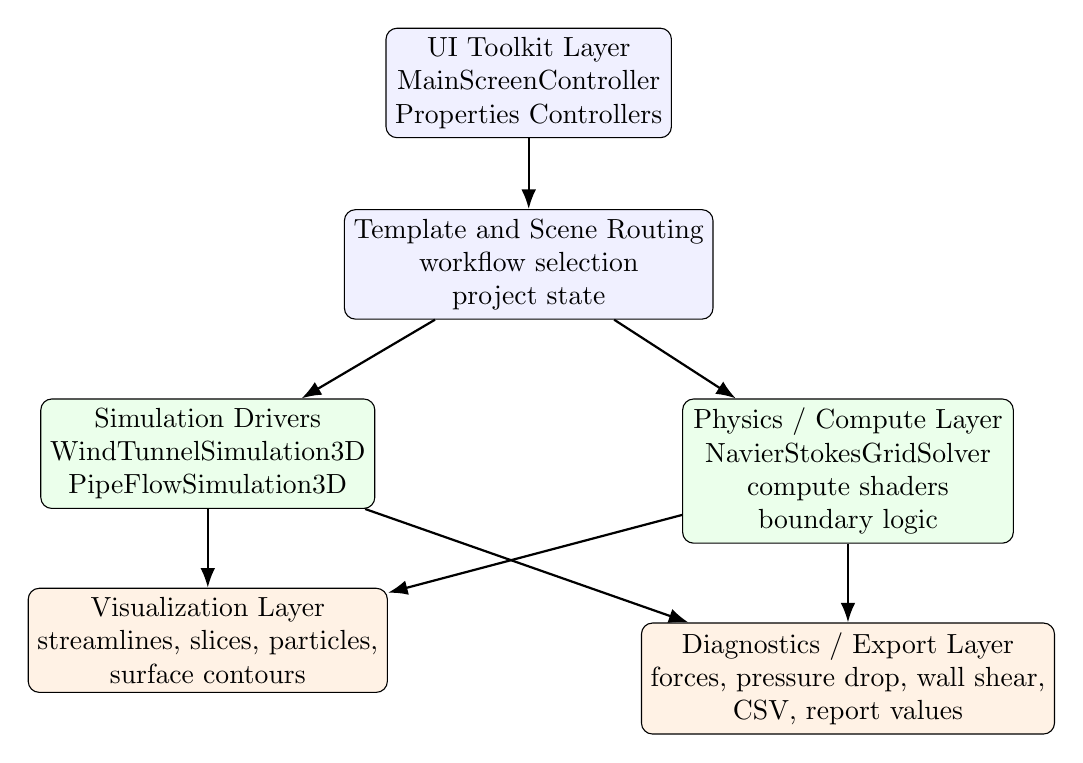
\begin{tikzpicture}[
node distance=0.9cm and 1.0cm,
box/.style={draw, rounded corners, align=center, minimum width=3.5cm, minimum height=0.95cm, fill=blue!6},
core/.style={draw, rounded corners, align=center, minimum width=4.2cm, minimum height=1.0cm, fill=green!8},
viz/.style={draw, rounded corners, align=center, minimum width=3.6cm, minimum height=0.95cm, fill=orange!10},
arrow/.style={-{Latex[length=2.5mm]}, thick}
]
\node[box] (ui) {UI Toolkit Layer\\MainScreenController\\Properties Controllers};
\node[box, below=of ui] (template) {Template and Scene Routing\\workflow selection\\project state};
\node[core, below left=1.0cm and -0.4cm of template] (sim) {Simulation Drivers\\WindTunnelSimulation3D\\PipeFlowSimulation3D};
\node[core, below right=1.0cm and -0.4cm of template] (solver) {Physics / Compute Layer\\NavierStokesGridSolver\\compute shaders\\boundary logic};
\node[viz, below=1.0cm of sim] (vis) {Visualization Layer\\streamlines, slices, particles,\\surface contours};
\node[viz, below=1.0cm of solver] (metrics) {Diagnostics / Export Layer\\forces, pressure drop, wall shear,\\CSV, report values};

\draw[arrow] (ui) -- (template);
\draw[arrow] (template) -- (sim);
\draw[arrow] (template) -- (solver);
\draw[arrow] (sim) -- (vis);
\draw[arrow] (solver) -- (vis);
\draw[arrow] (solver) -- (metrics);
\draw[arrow] (sim) -- (metrics);
\end{tikzpicture}
\caption{High-level architecture of the current FluidWorks runtime}
\label{fig:highlevel}
\end{figure}

\section{Primary Solver Summaries}
Understanding the current implementation is easiest when focusing on the solver stacks directly, so the report now provides a short description of each active solver path instead of reproducing their entire source listings.

\subsection{External Aero Solver Stack}
\texttt{Assets/Scripts/Sim3D/WindTunnel/WindTunnelSimulation3D.cs} orchestrates the external-aero runtime: it validates settings, controls playback, keeps the explicit \texttt{flowAxis}, updates vehicle reference data through \texttt{TryGetVehicleReferenceFrame}, and dispatches compute iterations to the physics layer while managing visualization mode switching. The solver layer consists of \texttt{Assets/Scripts/Physics/WindTunnel/NavierStokesGridSolver.cs}, which handles the grid buffers, obstacle/voxel masks, pressure projection, and divergence diagnostics before passing the updated velocity field to visualization components. The heavy lifting is performed in \texttt{Assets/Resources/Compute/WindTunnel/NavierStokes3D.compute}, whose kernels advance the grid solve, advect particles, and step the streamline seeds while honoring moving-ground and wheel-proxy boundary behaviors. The visualization support handles solver-weighted streamlines, field slices, particle wakes, and surface pressure contours, with \texttt{Assets/Scripts/Visualization/WindTunnel/StreamlineFieldRenderer.cs}, \texttt{Assets/Scripts/Visualization/WindTunnel/FlowFieldSliceRenderer.cs}, and \texttt{Assets/Scripts/Visualization/WindTunnel/FlowParticleSystem.cs} presenting the numeric fields clearly to the user.

\subsection{Internal Flow Solver Stack}
\texttt{Assets/Scripts/Sim3D/PipeFlow/PipeFlowSimulation3D.cs} drives the internal-flow template. It uses mesh bounds to carve the computational domain, enforces grid resolution controls, steps the GPU solver, and caches diagnostics such as mean velocity, pressure drop, divergence error, and wall shear. The \texttt{BoundaryConditionManager.cs} component registers inlet and outlet openings, assigns boundary types for each detected opening, and ensures the solver only runs once the assignments are valid. Surface-oriented diagnostics now also feed back through \texttt{Assets/Scripts/Visualization/InternalFlow/InternalSurfacePressureVisualizer.cs}, which shades model geometry using pressure or friction gradients tied to the solver field. This workflow preserves the separation between numeric accuracy and readable surface cues while keeping the solver data explicit.

\subsection{Vehicle, Obstacle, and UI Support}
\texttt{Assets/Scripts/Physics/WindTunnel/ObstacleVoxelizer.cs} rasterizes loaded geometry into obstacle masks for both the solver and the moving-ground proxies, while the UI layer — chiefly \texttt{Assets/Scripts/UI/MainScreenController.cs} and \texttt{Assets/Scripts/UI/WindTunnel/WindTunnelPropertiesController.cs} — routes template selection, exposes mode-specific sliders/toggles, and keeps diagnostics and exports synchronized with the active simulation. This updated summary highlights the main solver-relevant paths without reproducing line-by-line source listings.

\section{Architectural Rationale}
The architecture deliberately separates orchestration, solving, rendering, and UI control. This separation matters because the simulation has to remain inspectable while still being extensible. If solver logic, model loading, visualization state, and UI code were tightly mixed, every new feature would risk destabilizing unrelated workflows. The present layout reduces that risk:
\begin{enumerate}
\item simulation drivers own the high-level state of a workflow,
\item solver and compute layers own numeric stepping,
\item visualization components consume field data and convert it into readable output,
\item UI controllers bind widgets to settings and diagnostics, and
\item reporting/export code sits at the edge of the system rather than inside the core solver loop.
\end{enumerate}

\section{Data Flow Through a Frame}
One useful way to understand the architecture is to view a single runtime frame:
\begin{enumerate}
\item the user modifies a setting or visualization mode through the UI,
\item the active simulation driver updates cached settings and validates prerequisites,
\item compute buffers are dispatched or reused for the next solve step,
\item updated velocity and pressure data become available to visualization systems,
\item renderers display streamlines, slices, particles, or surface contours, and
\item diagnostics and export data are refreshed for the panel or report layer.
\end{enumerate}

\chapter{External Aero: Current Wind-Tunnel Stack}
\section{Runtime Flow}
The external-aero path is the primary solver workflow in the repository. The main driver is \texttt{WindTunnelSimulation3D}, which controls simulation state, settings, playback, visualization mode switching, and links to solver and visualization components. The project notes define a few implementation constraints that are important for the current design:
\begin{enumerate}
\item The tunnel flow axis is kept explicit through \texttt{flowAxis}; longest-axis heuristics are intentionally avoided.
\item \texttt{useRawSolverDataOnly} remains a debug toggle and is not the normal default.
\item Vehicle-aware values live under \texttt{WindTunnelSettings.vehicle} and affect derived estimates rather than the core field solve.
\item Shared vehicle reference-frame data is centralized in \texttt{TryGetVehicleReferenceFrame}.
\end{enumerate}

\section{Wind-Tunnel Pipeline}
Figure \ref{fig:windpipeline} summarizes the current flow of data through the external-aero stack.

    \begin{figure}[H]
        \centering
        \resizebox{\textwidth}{!}{
        \begin{tikzpicture}[
        node distance=0.8cm and 0.8cm,
        step/.style={draw, rounded corners, minimum width=3.0cm, minimum height=1.0cm, align=center, fill=cyan!8},
        arrow/.style={-{Latex[length=2.5mm]}, thick}
        ]
        \node[step] (import) {Runtime Model Import\\OBJ / STL / GLB / GLTF};
        \node[step, right=of import] (voxel) {Obstacle Voxelization\\ObstacleVoxelizer};
        \node[step, right=of voxel] (solver) {GPU Grid Solve\\NavierStokesGridSolver\\NavierStokes3D.compute};
        \node[step, below=of voxel] (driver) {WindTunnelSimulation3D\\settings, time step,\\mode switching};
        \node[step, left=of driver] (vehicle) {Vehicle Reference Frame\\ CG, axle, wheel,\\ ground reference};
        \node[step, right=of driver] (viz) {Visualization\\streamlines, slices, particles,\\surface pressure};
        \node[step, below=of driver] (metrics) {Diagnostics and Estimates\\drag, vertical aero force,\\moments, top speed};

        \draw[arrow] (import) -- (voxel);
        \draw[arrow] (voxel) -- (solver);
        \draw[arrow] (driver) -- (solver);
        \draw[arrow] (vehicle) -- (driver);
        \draw[arrow] (solver) -- (viz);
        \draw[arrow] (driver) -- (viz);
        \draw[arrow] (solver) -- (metrics);
        \draw[arrow] (vehicle) -- (metrics);
        \end{tikzpicture}
        }
        \caption{Current wind-tunnel data flow in FluidWorks}
        \label{fig:windpipeline}
    \end{figure}

\section{Visualization Contract}
The wind-tunnel path is not a single generic renderer. It uses distinct visualization modes with different interpretation goals.

\begin{table}[H]
\centering
\caption{Current external-aero visualization contract}
\label{tab:vizcontract}
\begin{tabular}{p{3.0cm}p{8.8cm}}
\toprule
\textbf{Mode} & \textbf{Current intent} \\
\midrule
Effects & Stylized but readable wake around a loaded vehicle \\
Streamlines & Solver-weighted path visualization for qualitative flow tracing \\
Velocity & Compact solver-driven slices and focused streamlines \\
Pressure & Model pressure view plus body-adjacent slice; not a full-screen slab \\
Surface Pressure & Additive body-only contour mode, kept separate from Pressure mode \\
\bottomrule
\end{tabular}
\end{table}

This distinction is important because the latest project state intentionally avoids flooding the scene with oversized planes or weakly related visual overlays. The renderers are organized so that each mode answers a specific question rather than repeating the same field in different colors.

\section{Streamline Rendering Quality}
The streamline system is particularly important in the current build. Repository instructions indicate that solver data remains the primary velocity source, with an analytical model used only as fallback support. Stable random seeding is preserved to avoid frame-to-frame flicker, and the line, travel, and threshold defaults are tuned to preserve wake readability instead of forcing unnaturally straight paths. This is a meaningful update because it shows that the project now treats visualization quality as part of the engineering workflow rather than as an afterthought.

\section{Engineering Outputs}
The external-aero workflow produces more than pictures. The current project distinguishes solver diagnostics from vehicle-aware estimates. Solver diagnostics include mean velocity, maximum velocity, pressure drop, wall shear, divergence error, and mean vorticity. Vehicle-aware outputs include drag force, vertical aerodynamic force, downforce, center of pressure, pitch/yaw/roll moments, axle loads, and estimated top speed. This distinction is useful because it separates directly computed field behavior from higher-level engineering interpretation.

\section{Why the Explicit Flow Axis Matters}
The repository notes emphasize that the tunnel flow axis must remain explicit through \texttt{WindTunnelSimulation3D.flowAxis}. This may appear like a small implementation rule, but it reflects a sound engineering decision. Heuristics such as ``use the longest model axis'' can fail when the imported geometry is asymmetrical, rotated, or intentionally non-vehicle-shaped. An explicit axis keeps the solver setup deterministic and makes the workflow easier to explain and validate.

\chapter{Internal Flow: Updated Pipeline}
\section{Current Direction}
The internal-flow module has evolved beyond a simple placeholder. The present \texttt{PipeFlowSimulation3D} driver uses a mesh-aware grid domain, internal opening detection, boundary assignment support, GPU compute execution, and surface-oriented diagnostics. This makes the internal-flow path much more aligned with the rest of the project's design philosophy: solver data should be visible, interpretable, and directly tied to the model.

\section{Internal-Flow Pipeline}
\begin{figure}[H]
\centering
\begin{tikzpicture}[
node distance=0.9cm and 0.8cm,
step/.style={draw, rounded corners, minimum width=3.1cm, minimum height=1.0cm, align=center, fill=green!9},
arrow/.style={-{Latex[length=2.5mm]}, thick}
]
\node[step] (mesh) {Loaded Pipe / Duct Mesh};
\node[step, right=of mesh] (domain) {Domain Bounds\\padding and grid setup};
\node[step, right=of domain] (openings) {BoundaryConditionManager\\opening detection\\inlet / outlet assignment};
\node[step, below=of domain] (solve) {PipeFlowSimulation3D\\GPU velocity, pressure,\\divergence updates};
\node[step, left=of solve] (diag) {Diagnostics\\flow rate, Reynolds,\\pressure drop, wall shear};
\node[step, right=of solve] (surface) {InternalSurfacePressureVisualizer\\pressure or friction contours};

\draw[arrow] (mesh) -- (domain);
\draw[arrow] (domain) -- (openings);
\draw[arrow] (openings) -- (solve);
\draw[arrow] (solve) -- (diag);
\draw[arrow] (solve) -- (surface);
\end{tikzpicture}
\caption{Updated internal-flow pipeline}
\label{fig:pipepipeline}
\end{figure}

\section{Recent Internal-Flow Changes}
The current internal-flow work introduces three practical improvements:
\begin{enumerate}
\item Boundary-condition handling is explicit through a dedicated manager rather than being hidden inside a generic flow preview.
\item Diagnostics are grouped around engineering quantities such as mean velocity, pressure drop, wall shear, divergence error, flow rate, and Reynolds number.
\item Surface rendering now supports pressure and friction contour views through \texttt{InternalSurfacePressureVisualizer}, making internal flow easier to interpret directly on the model surface.
\end{enumerate}

These changes are significant because the old style of reporting could describe internal flow only as a secondary feature. The current codebase now justifies discussing it as an active workflow with clear inputs, outputs, and visualization logic.

\section{Boundary Assignment as a Workflow Requirement}
The internal-flow path introduces a constraint that is especially important for usability: the solver should not continue as if the setup is valid when the boundary assignments are incomplete. In practice, this means the software has to detect openings, let the user classify them, and prevent misleading results when the flow direction is under-specified. This is better engineering behavior than silently inventing openings or always assuming the first opening is an inlet.

\section{Surface Pressure and Surface Friction Modes}
The new internal surface visualizer is useful from both an engineering and a presentation standpoint. Pressure contours help the user identify stagnation, suction, or loading patterns along the internal geometry. Friction contours make it easier to discuss boundary-layer interaction and where flow is actively working against the surface. In a report or viva presentation, these views are easier to explain than raw scalar arrays, which is precisely why they belong in the product.

\chapter{User Interface and Workflow}
\section{UI Structure}
The UI layer is managed primarily through \texttt{MainScreenController} and mode-specific properties controllers. The home screen routes the user into the selected workflow, after which the appropriate property panel binds to the active simulation. The wind-tunnel and pipe-flow interfaces each expose settings tied closely to their runtime drivers instead of relying on one generic panel for every mode.

\section{Typical User Workflow}
\begin{enumerate}
\item Launch the application and select a simulation template.
\item Import a geometry file if the selected mode requires one.
\item Adjust mode-specific settings in the properties panel.
\item Run the simulation and inspect flow behavior using the selected visualization mode.
\item Read diagnostics from the UI and export results if needed.
\end{enumerate}

\begin{figure}[H]
\centering
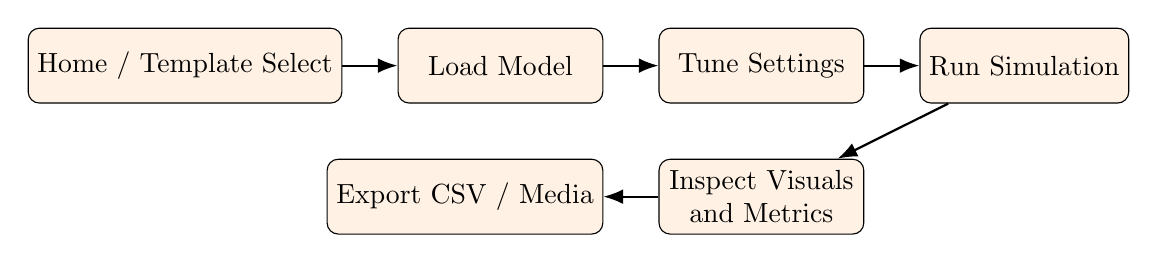
\begin{tikzpicture}[
node distance=0.7cm and 0.7cm,
block/.style={draw, rounded corners, minimum width=2.6cm, minimum height=0.95cm, align=center, fill=orange!11},
arrow/.style={-{Latex[length=2.5mm]}, thick}
]
\node[block] (home) {Home / Template Select};
\node[block, right=of home] (load) {Load Model};
\node[block, right=of load] (set) {Tune Settings};
\node[block, right=of set] (run) {Run Simulation};
\node[block, below=of set] (view) {Inspect Visuals\\and Metrics};
\node[block, left=of view] (export) {Export CSV / Media};

\draw[arrow] (home) -- (load);
\draw[arrow] (load) -- (set);
\draw[arrow] (set) -- (run);
\draw[arrow] (run) -- (view);
\draw[arrow] (view) -- (export);
\end{tikzpicture}
\caption{Typical user workflow in FluidWorks}
\label{fig:userworkflow}
\end{figure}

\chapter{Algorithmic Workflow}
\section{Initialization Phase}
Before a simulation can run, FluidWorks performs several setup tasks. These typically include:
\begin{enumerate}
\item finding or loading the target geometry,
\item determining domain bounds and padding,
\item creating or resizing compute buffers,
\item identifying obstacle or fluid regions,
\item preparing boundary information, and
\item selecting the visualization mode.
\end{enumerate}

\section{Per-Frame Simulation Loop}
At runtime, the solver loop can be summarized as follows:
\begin{enumerate}
\item check whether the simulation is initialized and not paused,
\item ensure prerequisites such as valid boundaries are satisfied,
\item clamp frame time to avoid unstable jumps,
\item execute one or more iterations per frame depending on quality settings,
\item update diagnostics from the resulting field, and
\item notify visualization systems that fresh data is ready.
\end{enumerate}

\section{Representative Pseudocode}
\begin{lstlisting}[language=C++,caption={High-level workflow pseudocode for FluidWorks},label={lst:pseudocode}]
Start Application
Load Home Screen
User selects simulation mode

if mode requires geometry then
    import model
    compute bounds
    prepare runtime scene objects
end if

initialize simulation driver
initialize solver buffers
bind UI controls to settings

while application is running do
    if user changes settings then
        update simulation configuration
    end if

    if simulation is active then
        validate prerequisites
        step solver
        refresh diagnostics
        update active visualizers
    end if

    if user requests export then
        capture images
        generate report output
    end if
end while
\end{lstlisting}

\chapter{Implementation Details}
\section{Runtime Model Import}
Runtime model import is essential because the project is meant for experimentation rather than hard-coded sample scenes alone. The import pipeline allows users to load geometry, inspect it in the scene, and feed it into different simulation templates. This is particularly useful for demonstrations where one model must be analyzed in multiple ways without rebuilding the application.

\section{BoundaryConditionManager in Internal Flow}
The \texttt{BoundaryConditionManager} is significant because it moves a critical setup task into an explicit component. In many student projects, boundary conditions remain hidden or hard-coded. Here, the project acknowledges that internal-flow correctness depends on boundary meaning. The manager therefore acts as a bridge between geometry interpretation and solver control.

\section{Report Generation}
The repository also contains a report generation pipeline that captures simulation views and injects diagnostics into a formatted template. This is an important product feature because it closes the loop from experimentation to communication. Engineers and students rarely stop at visual inspection; they must present findings. A system that generates report-ready assets has practical value beyond the simulation itself.

\chapter{Results Interpretation and Discussion}
\section{What the User Learns from the Visualizations}
The main value of FluidWorks lies in how quickly it turns numeric state into intuition. Streamlines show path tendency. Slices reveal local field variation. Surface pressure gives body-coupled loading cues. Particles and stylized effects make motion easier to perceive in demonstrations. Internal friction contours draw attention to where the surface is interacting most strongly with the fluid. Together, these allow the user to form a narrative around the model rather than staring at isolated numbers.

\section{External Aero Discussion}
For an external vehicle-like body, the user can interpret several common patterns:
\begin{enumerate}
\item a stagnation region near the front where pressure increases,
\item acceleration around curved or narrowed regions,
\item wake formation behind the body,
\item local asymmetry when yaw or custom inlet direction is applied, and
\item changes in derived drag or balance estimates when the geometry and settings vary.
\end{enumerate}

\section{Internal Flow Discussion}
For an internal pipe or duct model, the user can inspect:
\begin{enumerate}
\item whether the assigned inlet and outlet produce the expected main path,
\item where the pressure drop concentrates,
\item whether turns or contractions create higher local friction,
\item whether visual flow remains continuous through the cavity, and
\item whether the reported Reynolds-style trends match qualitative expectations.
\end{enumerate}

\chapter{Applications and Future Enhancements}
\section{Potential Applications}
FluidWorks can be applied in several contexts:
\begin{enumerate}
\item classroom demonstration of flow concepts,
\item early-stage shape comparison,
\item internal passage or duct visualization,
\item presentation support during mini-project evaluation, and
\item interactive proof-of-concept work for future engineering products.
\end{enumerate}

\section{Future Enhancements}
Several extensions would further strengthen the platform:
\begin{enumerate}
\item higher-fidelity turbulence approximations or selectable solver presets,
\item richer geometry preprocessing and repair,
\item automated benchmark scenes with known expected trends,
\item more export formats for diagnostics and images,
\item AI-assisted recommendations for setup or interpretation, and
\item improved comparative studies across multiple design variants.
\end{enumerate}

\chapter{Recent Repository Improvements}
\section{Present-Day Changes Reflected in This Report}
Compared with the older report, the current repository state shows several changes that needed to be reflected explicitly:
\begin{enumerate}
\item The project identity has moved from the old \LegacyProductName{} naming to FluidWorks, even though some namespaces remain unchanged.
\item The wind-tunnel path now has clearer design rules around flow-axis handling, vehicle orientation, moving-ground proxies, and solver diagnostics.
\item External-aero visualization modes are more deliberate and less redundant.
\item Internal-flow analysis is stronger, with better boundary management and new surface-based rendering.
\item The report no longer needs large source-code listings to explain the project because the architecture is clearer and more modular.
\end{enumerate}

\section{Why Code Listings Were Reduced}
The previous report relied on long source-code appendices. That made the document heavy without necessarily improving understanding. In this revised version, the main chapters still prioritize explanation and architecture, but representative code listings are restored in the appendix because the academic submission needs visible implementation evidence. The report therefore:
\begin{enumerate}
\item references only the main technical files,
\item explains how those files connect to each other,
\item shows architecture using diagrams,
\item includes selected sample listings from the actual project, and
\item leaves the full repository as the source of complete implementation detail.
\end{enumerate}

This produces a report that is easier to read, easier to present, and more aligned with the current maturity of the codebase.

\chapter{Validation and Testing}
\section{Validation Approach}
The project is intended for real-time educational and exploratory use, so validation focuses on behavioral correctness, visual stability, and physically sensible trend response. For the wind-tunnel path, the repository includes a QA checklist that verifies stable baseline flow, clean mode switching, response to yaw and custom wind directions, turbulence stress behavior, and visual containment near the body.

\section{Compile and Build Validation}
Repository guidance also requires a Unity batch compile check after non-trivial wind-tunnel changes and a Windows batch build after the compile check passes. This is an important part of project discipline because Unity projects can fail at compile, serialization, scene binding, or build-export stages even when a single script appears correct in isolation.

\section{Current Validation Targets}
\begin{table}[H]
\centering
\caption{Representative validation targets in the current repository}
\label{tab:validation}
\begin{tabular}{p{3.2cm}p{4.9cm}p{4.8cm}}
\toprule
\textbf{Workflow} & \textbf{What is checked} & \textbf{Expected outcome} \\
\midrule
External Aero & Mode switching, yaw response, custom wind direction, turbulence stress & Stable visuals, clear mode replacement, no screen-filling artifacts \\
External Aero & Solver diagnostics & Readable values for divergence error and mean vorticity \\
Internal Flow & Boundary assignment and opening detection & Valid inlet and outlet setup before analysis \\
Internal Flow & Pressure and friction contours & Surface feedback remains tied to computed field behavior \\
UI / Workflow & Template selection, property binding, export triggers & Controls map correctly to active simulation state \\
\bottomrule
\end{tabular}
\end{table}

\section{Limitations}
The present build still has clear limitations:
\begin{enumerate}
\item It is not a replacement for high-fidelity commercial CFD packages.
\item Numerical accuracy is secondary to interactive readability and engineering intuition.
\item Very large geometry, high grid resolution, or missing compute-shader support can reduce performance.
\item Some workflows are more mature than others, with the wind-tunnel path remaining the most developed.
\end{enumerate}

\chapter{Conclusion}
FluidWorks has developed into a practical real-time CFD-style visualization platform with a clear architectural center: a maintained external-aero wind-tunnel workflow supported by runtime geometry loading, GPU solving, and visualization modules that are tuned for readability. The latest repository state also shows meaningful growth in internal-flow analysis, especially through boundary-condition handling and surface contour rendering.

This updated report reflects those changes directly. It replaces the older code-heavy presentation with a current architecture-oriented document that explains the system using the main files, workflow diagrams, and present-day engineering behavior. In its current state, FluidWorks is best understood as an interactive educational and concept-analysis platform that bridges the gap between static classroom explanation and expensive offline CFD workflows.

\begin{thebibliography}{9}
\bibitem{anderson}
John D. Anderson,
\textit{Computational Fluid Dynamics: The Basics with Applications},
McGraw-Hill, 1995.

\bibitem{versteeg}
H. K. Versteeg and W. Malalasekera,
\textit{An Introduction to Computational Fluid Dynamics: The Finite Volume Method},
Pearson, 2007.

\bibitem{white}
Frank M. White,
\textit{Fluid Mechanics},
McGraw-Hill, 2016.

\bibitem{unity}
Unity Technologies,
\textit{Unity Manual and Compute Shader Documentation},
\url{https://docs.unity3d.com/}.
\end{thebibliography}

\begin{appendices}
    \chapter{Wind-Tunnel Runtime Driver}
    This appendix provides the wind-tunnel driver excerpt that anchors the reader to the project’s solver orchestration.

    \lstinputlisting[language={[Sharp]C},firstline=1,lastline=80,caption={Excerpt from the beginning of the wind-tunnel runtime driver (single-page view)},label={lst:winddriver}]{appendix_src/WindTunnelSimulation3D.cs}
    \noindent\textit{Listing truncated after the first page; the remaining implementation resides in the repository.}

    \chapter{Supplementary Explanation}
    \section{Listing Selection}
    The wind-tunnel driver listing was chosen because it shows the high-level simulation orchestration, validation checks, and visualization-mode handling described earlier in the report.

    \section{How the Listing Supports the Report}
    This single listing keeps the appendix concise while still grounding the architecture narrative in real implementation. The reader sees how the simulation driver validates state, depends on solver diagnostics, and interacts with visualization helpers, which reinforces the explanations in Chapters 2–7.

\end{appendices}

\end{document}
